O modelo que vamos discutir nessa subseção foi inicialmente introduzido por Fortuin e Kasteleyn em \cite{fortuin1972random} e é conhecido como ``Modelo de Percolação FK'' (ou ``\textit{Random Cluster Model}'').

Seja $\LX^d = (\ZX^d, \text{E}^d)$ reticulado $d$ dimensional, onde $\ZX^d$ é conjunto de vértices e $\text{E}^d$ é conjunto de elos, tal que, para $x, y \in \ZX^d$, $\text{E}^d = \left\{(x, y) \in \ZX^d \times \ZX^d : \sum_{i = 1}^{d} |x_i - y_i| = 1\right\}$. Defina o grafo \textit{finito} $\mathbb{G} = (\text{V}, \text{E})$, onde $\text{V} \subset \ZX^d$ é conjunto de vértices e $\text{E} \subset \text{E}^d$ é conjunto de elos $e = (x, y)$, tal que $x, y \in \text{V}$.

Inicialmente, defina um espaço de probabilidade $(\Omega, \FX, \mu)$, onde $\Omega = \{0, 1\}^{|\text{E}|}$, com $\omega = (\omega_e: e \in \text{E}) \in \Omega$, tal que  $\omega_e = 0$ para elo $e$ ``fechado'' e $\omega_e = 1$ para elo $e$ ``aberto'', $\FX = \mathcal{P}(\Omega)$ e, para $p \in [0, 1]$ e $q \in (0, +\infty)$,
\begin{align*}
\mu_{\mathbb{G}, p, q}(\omega) = \frac{p^{|\omega|} (1 - p)^{|\text{E}| - |\omega|} q^{k(\omega)}}{\text{Z}_{\mathbb{G}, p, q}},
\end{align*}
onde $|\omega| = \sum_{e \in \text{E}} \omega_e$, $k(\omega)$ é o número de componentes conexas em $\omega$ (incluindo vértices isolados) e
\begin{align*}
Z_{\mathbb{G}, p, q} = \sum_{\omega \in \Omega} p^{|\omega|} (1 - p)^{|\text{E}| - |\omega|} q^{k(\omega)}
\end{align*}
é constante normalizadora.

Note que, para $q = 1$, $\mu_{\mathbb{G}, p, q}(\omega)$ é medida produto Bernoulli e obtemos o modelo de percolação independente com parâmetro $p$.

Perceba, também, que a medida $\mu$, como acabamos de descrever, é medida monótona. De maneira geral, temos a seguinte definição:

\begin{mydef} \label{def-medidamonotona}
	Uma medida $\mu$ em $\{0, 1\}^{|\text{E}|}$ é \textit{monótona} se, para qualquer $e \in \text{E}$, qualquer $\text{F} \subset \text{E}$ e para qualquer $\xi, \zeta \in \{0, 1\}^{|\text{F}|}$ satisfazendo $\xi \leq \zeta$, $\mu(\omega_e = \xi_e, \forall e \in \text{F}) > 0$ e $\mu(\omega_e = \zeta_e, \forall e \in \text{F}) > 0$, temos que\vspace{-6pt}
	\begin{align*}
		\mu(\omega_e = 1 \,|\, \omega_e = \xi_e, \forall e \in \text{F}) \leq \mu(\omega_e = 1 \,|\, \omega_e = \zeta_e, \forall e \in \text{F}).
	\end{align*}
\end{mydef}

Medidas como as da Definição \ref{def-medidamonotona} gozarão de versões estendidas de alguns dos resultados das Seções \ref{How-to-prove} e \ref{Bernoulli-percolation}, discutidas ao longo dessa subseção. 

Agora, a fim de estender o modelo que acabamos de descrever para um conjunto com volume infinito, defina, para $\Omega = \prod_{e \in \text{E}^d} \{0, 1\}$, com $\omega, \xi \in \Omega$ e $\FX = \sigma($cilindros finito-dimensionais$)$,
\[\omega_{\mathbb{G}}^{\xi}(e) = 
\begin{cases}
\omega_e & \text{se } e \in \mathbb{G} \\
\xi_e & \text{caso contrário},
\end{cases}
\]
com $\xi$ agindo como \textit{boundary condition} (ou ``condição de fronteira''). Assim, para $\Omega_{\mathbb{G}}^{\xi}$ subconjunto \textit{finito} de $\Omega$, tal que $\omega_e = \xi_e$, $\forall e \in \text{E}^d \, \backslash \, \text{E}$,
\[\mu_{\mathbb{G}, p, q}^\xi(\omega) = 
\begin{cases}
\frac{p^{|\omega|} (1 - p)^{|\text{E}| - |\omega|} q^{k(\omega, \xi)}}{\text{Z}_{\mathbb{G}, p, q}^{\xi}} & \text{se } \omega \in \Omega_{\mathbb{G}}^{\xi} \\
0 & \text{caso contrário},
\end{cases}
\]
onde $k(\omega, \xi)$ é o número de componentes conexas em $\omega$ que intersectam com $\mathbb{G}$ e
\begin{align*}
\text{Z}_{\mathbb{G}, p , q}^{\xi} = \sum_{\omega \in \Omega_{\mathbb{G}}^{\xi}} p^{|\omega|} (1 - p)^{|\text{E}| - |\omega|} q^{k(\omega, \xi)}.
\end{align*} 

Em particular, estamos interessados nas medidas $\mu_{\mathbb{G}, p, q}^0$ e $\mu_{\mathbb{G}, p, q}^1$. A primeira delas implica que, a não ser pelas conexões dentro de $\mathbb{G}$, os vértices de $\partial\text{V}$ não estão conectados; ao passo que, na segunda, todos os vértices $x \in \partial\text{V}$ estão conectados.

Por fim, a ferramenta que vamos utilizar para argumentar em favor da extensão que gostaríamos de propor para definir uma medida $\mu_{\ZX^d, p, q}^{\xi}$ é chamada de \textit{Thermodynamic limit}, e é apresentada a seguir. Para isso, defina $\Lambda_n \colonequals [-n, n]^d$, com $n \in \NX$.

\begin{mythm}[\textit{Thermodynamic limit}] \label{thm:tl}
	Seja $p \in [0, 1]$, $q \in [1, +\infty)$ e $\mathbf{\Lambda} = (\Lambda_n)_{n \in \NX}$ uma sequência crescente de caixas tal que $\Lambda_n \rightarrow \ZX^d$, quando $n \rightarrow +\infty$. Então, para $\xi = 0, 1$, 
	\begin{enumerate}[a.]
		\item O limite
		\begin{align*}
		\mu_{\ZX^d, p, q}^{\xi} = \lim_{n \rightarrow +\infty} \mu_{\Lambda_n, p, q}^{\xi}
		\end{align*}
		existe e independe da escolha de $\mathbf{\Lambda}$.
		\item Vale que $\mu_{\ZX^d, p, q}^0 \leq \mu_{\ZX^d, p, q}^1$, no sentido de que $\mu_{\ZX^d, p, q}^0(A) \leq \mu_{\ZX^d, p, q}^1(A)$, para todo $A \in \FX$ evento crescente (chamado de ``ordem estocástica de medidas'').
	\end{enumerate}
\end{mythm}

A demostração do Teorema \ref{thm:tl} não será feita, porém, é possível encontrá-la em  \cite{grimmett2004random} (Thm. 4.19, ``a'' e ``c'').

Agora, de maneira similar ao que fizemos na Seção \ref{Bernoulli-percolation}, podemos definir o ponto crítico como ${p_c}^{\xi}(q) = \sup\{p: \theta^{\xi}(p, q) = 0\}$ com $\xi \in \{0, 1\}$, tal que $\theta^{\xi}:[0, 1] \times [1, +\infty) \longrightarrow [0, 1]$ é função que mapeia $(p, q) \mapsto \mu_{\ZX^d, p, q}^{\xi}(|C_0(\omega)| = +\infty)$. Além disso, como $\mu_{\ZX^d, p, q}^0 = \mu_{\ZX^d, p, q}^1$ para quase todo $p \in [0, 1]$ (em \cite{grimmett2004random}, Sec. 5.1), $\theta^0(p, q) = \theta^1(p, q)$ para quase todo $p \in [0, 1]$ $-$ já que $\theta^{\xi}(p, q)$ é não-decrescente em $p$ (também em \cite{grimmett2004random}, Sec. 5.1). Dessa forma, denotamos $p_c(q) = {p_c}^0(q) = {p_c}^1(q)$.

O teorema apresentado a seguir, que determina o ponto crítico para o modelo de Percolação FK em $\ZX^2$ foi inicialmente provado em \cite{beffara2012self} (com demonstrações alternativas em \cite{duminil2016phase} e \cite{duminil2018new}). Esse é um teorema ``novo'', no sentido de que ele generaliza o resultado para $q \geq 1$; ao passo que, antes, apenas os casos onde $q = 1$, $q = 2$ ou $q$ ``muito grande'' haviam sido demonstrados.

\begin{mythm}[Beffara, Duminil-Copin] \label{thm:pc}
	Para o modelo de Percolação FK em $\ZX^2$ com $q \in [1, +\infty)$,
	\begin{align*}
	p_c(q) = \frac{\sqrt{q}}{1 + \sqrt{q}}.
	\end{align*}
\end{mythm}

Porém, antes da demonstração (parcial $-$ já que ela depende fortemente dos que foi desenvolvido em \cite{duminil2019sharpdecisiontree}) do Teorema \ref{thm:pc}, são necessários alguns resultados intermediários.

\begin{mylem}[Desigualdade de FKG] \label{FKG-geral}
	Sejam $X$, $Y$ variáveis aleatórias crescentes e limitadas e $\mu$ medida monótona, então
	\begin{align*}
		\EX_{\mu}(X \cdot Y) \geq \EX_{\mu}(X) \cdot \EX_{\mu}(Y). 
	\end{align*}
\end{mylem}

Note que o Lema \ref{FKG-geral} é uma generalização do já apresentado (e demonstrado) Lema \ref{fkg-esp}. A demonstração dessa versão mais geral, que não será feita aqui, pode ser encontrada em \cite{grimmett2004random} (Thm. 2.16). Dois corolários imediados, apresentados a seguir, serão úteis mais tarde.

\begin{mycol} \label{col-fkg-geral}
	Sejam $A$, $B$ eventos crescentes, então
	\begin{align*}
	\mu(A \cap B) \geq \mu(A) \cdot \mu(B).
	\end{align*}
\end{mycol}

A demonstração do Corolário \ref{col-fkg-geral} é idêntica à que foi feita para o Corolário \ref{fkg}.

\begin{mycol}(Truque da raiz quadrada) \label{col-trq}
	Sejam $A_1, \cdots, A_n$ eventos crescentes e com mesma probabilidade. Defina $A = \bigcup_{i=1}^{n}A_i$. Então
	\begin{align*}
		\mu(A_1) \geq 1 - (1 - \mu(A))^{\frac{1}{n}}.
	\end{align*}
\end{mycol}

\texttt{Demonstração:}

Veja que
\begin{align*}
	1 - \mu\left(\bigcup_{i = 1}^n A_i\right) \overset{\phantom{\text{FKG}}}{=} \mu\left(\bigcap_{i=1}^n {A_i}^c\right) &\overset{\text{FKG}}{\geq} \prod_{i=1}^n \mu\left({A_i}^c\right) \\
			   &\overset{\phantom{\text{FKG}}}{=} \left(1 - \mu(A_1)\right)^n
\end{align*}
já que, por hipótese, $\mu(A_i) = \mu(A_j)$, $\forall i \neq j$; sendo assim, $\mu(A_1) \geq 1 - (1 - \mu\left(\bigcup_{i = 1}^n\right))^{\frac{1}{n}}$.\hspace{\fill}\qed

\begin{mypro} \label{unicidade-cluster}
	No modelo de Percolação FK em $\ZX^2$, para todo $p \in (p_c, 1]$, $q \in [1, +\infty)$ e $\xi \in \{0, 1\}$, vale que $\mu_{\ZX^d, p, q}^{\xi}(\{\omega \in \Omega : \text{N}(\omega) = 1\}) = 1$, onde $\text{N}(\omega)$ conta o número de aglomerados abertos de tamanho infinito em $\omega$. 
\end{mypro}

O que a Proposição \ref{unicidade-cluster} nos diz é que, se $\theta^{\xi}(p, q) > 0$, existe, quase certamente, aglomerado único de elos abertos. Esse resultado também não será provado aqui; entretanto, é possível encontrar sua demonstração em \cite{grimmett2004random} (Thm. 5.99).

\begin{mypro} \label{pro:propto}
	Se $\omega \sim \mu_{\mathbb{G}, p, q}^0$, então $\omega^{\star} \sim \mu_{\mathbb{G}^{\star}, p^{\star}, q^{\star}}^1$, onde $\omega^{\star}$ é uma configuração no reticulado dual com $\mathbb{G}^{\star} = (\text{V}^{\star}, \text{E}^{\star})$, tal que $q^{\star} = q$ e $p^{\star}$ respeita
	\begin{align}\label{p_dual_fk}
	p^{\star} = \frac{(1 - p) \, q}{(1 - p) \, q + p}, \text{ ou, de maneira equivalente } \frac{p^{\star} \, p}{(1 - p^{\star})(1 - p)} = q.
	\end{align}
\end{mypro}

\texttt{Demonstração:}

Seja $\mathbb{G} = (\text{V}, \text{E})$ grafo finito. Nesse caso, por definição, 
\begin{align} \label{eq:propto}
\mu_{\mathbb{G}, p, q}^0 \propto \left(\frac{p}{1 - p}\right)^{|\omega|} q^{k(\omega, 0)}.
\end{align}

Porém, note que $|\omega| = |\text{E}| - |\omega^{\star}|$ e $k(\omega, 0) = h(\omega^{\star})$, onde $h(\cdot)$ é a função que conta as faces de um grafo planar conectado. A Figura \ref{fig-dual-FK} nos ajuda a ter uma ideia de o porquê a última afirmação é verdadeira. 

\begin{figure*}[!htbp]
	\centering
	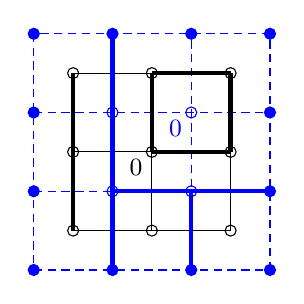
\begin{tikzpicture}[scale = 1.00]

	\node[black] at (-0.20, -0.20) {{\small $0$}};
	\draw[solid, black] (-1, 0) -- (1, 0);
	\draw[solid, black] (-1, 1) -- (1, 1);
	\draw[solid, black] (-1,-1) -- (1,-1);
	\draw[solid, black] (-1,-1) -- (-1,1);
	\draw[solid, black] ( 1,-1) -- (1, 1);
	\draw[solid, black] ( 0,-1) -- (0, 1);
	\draw[black] ( 0, 0) circle (2pt);
	\draw[black] ( 1, 0) circle (2pt);
	\draw[black] (-1, 0) circle (2pt);
	\draw[black] ( 0, 1) circle (2pt);
	\draw[black] ( 1, 1) circle (2pt);
	\draw[black] (-1, 1) circle (2pt);
	\draw[black] ( 0,-1) circle (2pt);
	\draw[black] ( 1,-1) circle (2pt);
	\draw[black] (-1,-1) circle (2pt);

	\node[blue] at (0.30, 0.30) {{\small $0$}};	
	\draw[densely dashed, blue] (-1.5, 0.5) -- (1.5, 0.5);
	\draw[densely dashed, blue] (-1.5,-0.5) -- (1.5,-0.5);
	\draw[densely dashed, blue] (-0.5,-1.5) -- (-0.5,1.5);
	\draw[densely dashed, blue] ( 0.5,-1.5) -- (0.5, 1.5);
	
	\draw[densely dashed, blue] (-1.5,-1.5) -- ( 1.5,-1.5);
	\draw[densely dashed, blue] ( 1.5,-1.5) -- ( 1.5, 1.5);
	\draw[densely dashed, blue] ( 1.5, 1.5) -- (-1.5, 1.5);
	\draw[densely dashed, blue] (-1.5, 1.5) -- (-1.5,-1.5);
	
	\draw[fill, blue] (-0.5,-1.5) circle (2pt);
	\draw[fill, blue] ( 0.5,-1.5) circle (2pt);
	\draw[fill, blue] (-0.5, 1.5) circle (2pt);
	\draw[fill, blue] ( 0.5, 1.5) circle (2pt);
	\draw[fill, blue] (-1.5,-0.5) circle (2pt);
	\draw[fill, blue] ( 1.5,-0.5) circle (2pt);
	\draw[fill, blue] (-1.5, 0.5) circle (2pt);
	\draw[fill, blue] ( 1.5, 0.5) circle (2pt);
	
	\draw[fill, blue] (-1.5,-1.5) circle (2pt);
	\draw[fill, blue] ( 1.5,-1.5) circle (2pt);
	\draw[fill, blue] (-1.5, 1.5) circle (2pt);
	\draw[fill, blue] ( 1.5, 1.5) circle (2pt);
	
	\draw[blue] (-0.5, 0.5) circle (2pt);
	\draw[blue] (-0.5,-0.5) circle (2pt);
	\draw[blue] ( 0.5, 0.5) circle (2pt);
	\draw[blue] ( 0.5,-0.5) circle (2pt);
	
	
	\draw[solid, black, ultra thick] (-1,-1) -- (-1,1);
	\draw[solid, black, ultra thick] ( 0, 0) -- ( 0,1);
	\draw[solid, black, ultra thick] ( 0, 0) -- ( 1,0);
	\draw[solid, black, ultra thick] ( 1, 1) -- ( 0,1);
	\draw[solid, black, ultra thick] ( 1, 1) -- ( 1,0);
	
	\draw[solid, blue, ultra thick] (-0.5,-1.5) -- (-0.5,1.5);
	\draw[solid, blue, ultra thick] (-0.5,-0.5) -- (1.5,-0.5);
	\draw[solid, blue, ultra thick] ( 0.5,-1.5) -- (0.5,-0.5);
\end{tikzpicture}
	\caption{Configuração $\omega$ definida em $\mathbb{G}$ (linha sólida) e configuração correspondente $\omega^{\star}$ definida em $\mathbb{G}^{\star}$ (linha tracejada).}
	\label{fig-dual-FK}
\end{figure*}

Além disso, pela Fórmula de Euler\footnote{Para qualquer grafo planar (conectado) com $|\text{V}|$ vértices, $|\text{E}|$ elos e $|\text{H}|$ faces, vale que $|\text{V}| - |\text{E}| + |\text{H}| = 2$.}, temos que $h(\omega^{\star}) = |\omega^{\star}| + k(\omega^{\star}, 1) + 1 - |\text{V}^{\star}|$. Assim, da Expressão \eqref{eq:propto}, podemos escrever
\begin{align*}
\mu_{\mathbb{G}, p, q}^0 &\propto \left(\frac{p}{1 - p}\right)^{|E| - |\omega^{\star}|} q^{|\omega^{\star}| + k(\omega^{\star}, 1) + 1 - |\text{V}^{\star}|} \\
&\propto \left(q \cdot \frac{1 - p}{p}\right)^{|\omega^{\star}|} \, q^{k(\omega^{\star}, 1)} \\
&= \left(\frac{p^{\star}}{1 - p^{\star}}\right)^{|\omega^{\star}|} \, q^{k(\omega^{\star}, 1)} \propto \mu_{\mathbb{G}^{\star}, p^{\star}, q^{\star}}^{1},
\end{align*}
o que conclui a prova.\hspace{\fill}\qed

\begin{mypro} \label{prop-HLFK}
	No modelo de Percolação FK, para todo $p \in (p_c, 1]$ e $q \in 
	[1, +\infty)$, vale que $\mu_{G, p, q}^0(\HL(n + 1, n)) \rightarrow 1$, quando $n \rightarrow +\infty$.
\end{mypro}

\texttt{Demonstração:}

Nessa prova, a fim de não sobrecarregar a notação, defina $\text{R}(n, m) \colonequals \left[-\frac{n}{2}, \frac{n}{2}\right] \times \left[-\frac{m}{2}, \frac{m}{2}\right]$; e, por consequência, $\HL(n, m) = \{\exists$ cruzamento horizontal em $\text{R(n, m)}\}$ (determine $\VL(n, m)$ de forma análoga). Assim, para $k < \frac{n}{2}$ e usando o Corolário \ref{col-trq}, temos
\begin{align*}
\mu_{\ZX^d, p, q}^0(\partial\Lambda_k \leftrightarrow \text{lado A de } \partial\Lambda_{\frac{n}{2}}) &\geq 1 - (1 - \mu_{\ZX^d, p, q}^0(\partial\Lambda_k \leftrightarrow \partial\Lambda_{\frac{n}{2}}))^{\frac{1}{4}} \\
&= 1 - \mu_{\ZX^d, p, q}^0(\partial\Lambda_k \not\leftrightarrow \partial\Lambda_{\frac{n}{2}})^{\frac{1}{4}}\\
&\geq 1 - \mu_{\ZX^d, p, q}^0(\partial\Lambda_k \not\leftrightarrow +\infty)^{\frac{1}{4}}.
\end{align*}
Agora, para $\text{R} \colonequals \text{R(n + 1, n)}$, note que
\begin{align*}
&\mu_{\ZX^d, p, q}^0\left(\left\{\partial{\Lambda_k}^{\phantom{\prime}}\left(-\frac{k}{2}, 0\right) \leftrightarrow \text{lado A de } \partial\text{R}\right\} \cap \right. \\ 
&\phantom{\mu_{\ZX^d, p, q}^0\left(\right.}\left. \left\{\partial{\Lambda_k}^{\prime}\left(\phantom{-}\frac{k}{2}, 0\right) \leftrightarrow \text{lado B de } \partial\text{R}\right\}\right) \geq 1 - 2\,\mu_{\ZX^d, p, q}^0(\partial\Lambda_k \not\leftrightarrow +\infty)^{\frac{1}{4}}, \numberthis \label{in-parcial-hn1}
\end{align*}
onde ${\Lambda_k}^{\prime}$ é uma caixa deslocada de $k$ unidades para o lado em relação à caixa $\Lambda_k$ (veja a Figura \ref{fig-duas-caixinhas}). Perceba que, para a desigualdade acima, utilizamos o fato de que $\mu_{\ZX^d, p, q}^0\left(\bigcap_{i = 1}^n A_i\right) \geq 1 - \sum_{i = 1}^n \mu_{\ZX^d, p, q}^0({A_i}^c)$, para qualquer sequência finita de eventos $\{A_i\}_{i = 1}^{n}$.

\begin{figure*}[!htbp]
	\centering
	\begin{tikzpicture}[scale = 0.75]

\draw[solid, black] (-4, -3) -- ( 4, -3);
\draw[solid, black] (-4,  3) -- ( 4,  3);
\draw[solid, black] (-4, -3) -- (-4,  3);
\draw[solid, black] ( 4, -3) -- ( 4,  3);

\draw [decorate, decoration = {brace, amplitude = 6pt, mirror}, xshift = 4pt, yshift = 0pt] (4, -3) -- (4, 3) node [black, midway, xshift = 14pt, yshift = 0pt] {\small $n$};

\draw [decorate, decoration = {brace, amplitude = 6pt, mirror}, xshift = 0pt, yshift = -4pt] (-4, -3) -- (4, -3) node [black, midway, xshift = 0pt, yshift = -14pt] {\small $n + 1$};

\draw[solid, black] (-1.5, -1) -- (-1.5, 1);
\draw[solid, black] (-1.5, -1) -- (0.5, -1);
\draw[solid, black] ( 0.5, -1) -- (0.5,  1);
\draw[solid, black] ( 0.5,  1) -- (-1.5, 1);
\node[black] at (-2, -0.9) {{\small $\Lambda_k$}};

\draw[solid, black] ( 1.5, -1) -- ( 1.5, 1);
\draw[solid, black] ( 1.5,  1) -- (-0.5, 1);
\draw[solid, black] (-0.5,  1) -- (-0.5,-1);
\draw[solid, black] (-0.5, -1) -- ( 1.5,-1);
\node[black] at ( 2, -0.9) {{\small ${\Lambda_k}^{\prime}$}};

\node[black] at ( 6.5, 0) {{\small (lado B)}};
\node[black] at (-6.5, 0) {{\small (lado A)}};

\draw[solid, thick, black] (-1.5, 0) to[out = 135, in = -45] (-4, 0);
\draw[solid, thick, black] ( 1.5, 0) to[out = -45, in = 135] ( 4, 0);

\draw[fill] (-1.5, 0) circle (2.68pt);
\draw[fill] (  -4, 0) circle (2.68pt);
\draw[fill] ( 1.5, 0) circle (2.68pt);
\draw[fill] (   4, 0) circle (2.68pt);

	\draw[black] ( 0,  0) circle (2.68pt);
\node[black] at (0, -.4) {{\scriptsize $(0, 0)$}};

%	\draw[solid, black] (-2, -2) -- ( 2, -2);
%	\draw[solid, black] ( 2, -2) -- ( 2,  2);
%	\draw[solid, black] ( 2,  2) -- (-2,  2);
%	\draw[solid, black] (-2,  2) -- (-2, -2);
%	
%	\draw[solid, black] (-4, -4) -- ( 4, -4);
%	\draw[solid, black] ( 4, -4) -- ( 4,  4);
%	\draw[solid, black] ( 4,  4) -- (-4,  4);
%	\draw[solid, black] (-4,  4) -- (-4, -4);
%	
%	\draw[dashed, black] (-2, -4) -- (-2, 4);
%	\draw[dashed, black] ( 2, -4) -- ( 2, 4);
%	\draw[dashed, black] (-4, -2) -- ( 4,-2);
%	\draw[dashed, black] (-4,  2) -- ( 4, 2);
%	
%	\draw[black] ( 0,  0) circle (3.35pt);
%	\node[black] at (0, -.5) {{\footnotesize $(0, 0)$}};
%	\node[black] at (-2.4, -1.65) {{\small $\Lambda_{k\phantom{2}}$}};
%	\node[black] at (-4.6, -3.65) {{\small $\Lambda_{2k}$}};
%	
%	\draw[fill] ( -1,  1) circle (3.35pt);
%	\draw[fill] ( -4,  1) circle (3.35pt);
%	
%	\draw[solid, thick, black] (-1, 1) to[out = 135, in = -45] (-4, 1);
%	
%	\draw [decorate, decoration = {brace, amplitude = 6pt, mirror}, xshift = 4pt, yshift = 0pt] (2, -2) -- (2, 2) node [black, midway, xshift = 14pt, yshift = 0pt] {\small $2k$};
%	
%	\draw [decorate, decoration = {brace, amplitude = 6pt, mirror}, xshift = 4pt, yshift = 0pt] (4, -4) -- (4, 4) node [black, midway, xshift = 14pt, yshift = 0pt] {\small $4k$};
	
\end{tikzpicture}
	\vspace{-12pt}
	\caption{Esboço da ocorrência do evento $\{\partial\Lambda_k(-\frac{k}{2}, 0) \leftrightarrow \text{lado A de } \partial\text{R}\} \cap \{\partial{\Lambda_k}^{\prime}(\frac{k}{2}, 0) \leftrightarrow \text{lado B de } \partial\text{R}\}$.}
	\label{fig-duas-caixinhas}
\end{figure*}

Pela Proposição \ref{unicidade-cluster}; i.e., usando o fato de que na região supercrítica o aglomerado aberto com tamanho infinito existe e é único (quase certamente), e empregando a cota determinada através da Expressão \eqref{in-parcial-hn1},
\begin{align*}
\liminf_{n\rightarrow+\infty}\mu_{\ZX^d, p, q}^0(\HL(n + 1, n)) \geq 1 - 2\,\mu_{\ZX^d, p, q}^0(\partial\Lambda_k \not\leftrightarrow +\infty)^{\frac{1}{4}} \overset{k \rightarrow +\infty}{\longrightarrow} 1,
\end{align*}
para todo $p > p_c$; o que conclui a demonstração.\hspace{\fill}\qed

Além disso, e como mencionado em parágrafos anteriores, alguns dos resultados já discutidos em outras seções podem ser estendidos para medidas monótonas; em particular, para $\mu_{\ZX^d, p, q}^{\xi}$. Nesse sentido, vale uma extensão do Teorema \ref{osss-inequality}, enunciada a seguir.

\begin{mythm} \label{osss-extended}
	Seja $n \in \NX$ e $\mu$ medida monótona em $[n]$. Fixe uma função Booleana crescente $f: \{0, 1\}^n \longrightarrow \{0, 1\}$ e um algoritmo $\text{\textbf{T}}$; então vale que
	\begin{align*}
		\VX_{\mu}(f(\omega)) \leq \sum_{i \in [n]}\delta_i(\text{\textbf{T}}) \, \text{Inf}_i^{\mu}(f(\omega)),
	\end{align*}
	onde $\delta_i(\text{\textbf{T}})$ é definido da mesma forma que foi feito para o Teorema \ref{osss-inequality}.
\end{mythm}

\par A demonstração do Teorema \ref{osss-extended}, que se não será feita aqui, pode ser encontrada em \cite{duminil2019sharpdecisiontree}. 

Como aplicação do Teorema \ref{osss-extended} temos que, como no Teorema \ref{exp-decay}, a probabilidade da origem estar conectada à borda de uma caixa de lado $2n$ decai, na região subcrítica do modelo considerado, exponencialmente rápido com $n$. O teorema abaixo nos dá um resultado desse tipo.

\begin{mythm} \label{exp-decay-extended}
	No modelo de Percolação FK em $\ZX^d$, com $q \geq 1$, vale que
	\begin{enumerate}
		\item Para $p < p_c$, existe $c_p > 0$ tal que para todo $n \geq 1$, $\mu_{\Lambda_n, p, q}^{1}(0 \leftrightarrow \partial\Lambda_n) \leq e^{-c_p \, n}$.
		\item Para $p > p_c$, existe $c > 0$ tal que $\mu_{\ZX^d, p, q}^{1}(|C_0(\omega)| = +\infty) \geq c \, (p - p_c)$.
	\end{enumerate}
\end{mythm}

A demonstração do Teorema \ref{exp-decay-extended}, similar ao Teorema \ref{exp-decay}, pode ser encontrada em \cite{duminil2019sharpdecisiontree}.

Finalmente, e de posse de todas essas ferramentas, podemos nos concentrar na demonstração do principal resultado dessa subseção, o Teorema \ref{thm:pc}.
\vspace{6pt}

\texttt{Demonstração (Teorema \ref{thm:pc}):}

Para a prova desse resultado, vamos dividir os casos em que $p_c(q) \geq \frac{\sqrt{q}}{1 + \sqrt{q}}$ e $p_c(q) \leq \frac{\sqrt{q}}{1 + \sqrt{q}}$; o que concluiria a demonstração. 

Primeiro, note que, para $p$ tal que $p = p^{\star}$ (chamado de ponto \textit{self-dual}, ou $p_{sd}$), vale que $p_{sd}(q) = \frac{\sqrt{q}}{1 + \sqrt{q}}$. De fato, usando a Expressão \eqref{p_dual_fk} para $p = p^{\star}$,
\begin{align*}
q = \frac{p^2}{(1 - p)^2}
\implies \frac{1}{\sqrt{q}} = \frac{1 - p}{p}
\implies \frac{1 + \sqrt{q}}{\sqrt{q}} = \frac{1}{p}
\implies \frac{\sqrt{q}}{1 + \sqrt{q}} = p \equalscolon p_{sd}(q).
\end{align*} 
Nesse caso, para $p = p_{sd}$,
\begin{align*}
\mu_{\mathbb{G}, p, q}^0(\HL(n + 1, n)) &\overset{\text{Prop. \ref{pro:propto}}}{=} 1 - \mu_{\mathbb{G}^{\star}, p^{\star}, q^{\star}}^1\left(\VL^{\star}\left(\left[\frac{1}{2}, n + \frac{1}{2}\right] \times \left[-\frac{1}{2}, n + \frac{1}{2}\right]\right)\right) \\
&\overset{\text{Teor. \ref{thm:tl}}}{\leq} \hspace{1pt} 1 - \mu_{\mathbb{G}^{\star}, p^{\star}, q^{\star}}^0\left(\VL^{\star}\left(\left[\frac{1}{2}, n + \frac{1}{2}\right] \times \left[-\frac{1}{2}, n + \frac{1}{2}\right]\right)\right),
\end{align*}
o que implica em, por invariância por translação e usando o fato de que $p = p^{\star}$,
\begin{align} \label{in:boundmeasure}
\mu_{\mathbb{G}, p, q}^1(\HL(n + 1, n)) \overset{\text{Similarmente}}{\geq} \frac{1}{2} \overset{\phantom{XXX}}{\geq} \mu_{\mathbb{G}, p, q}^0(\HL(n + 1, n)), ~\forall n \in \NX.
\end{align}

Agora, sob o resultado da Proposição \ref{prop-HLFK}, que diz que $\forall p > p_c$, $\mu_{\mathbb{G}, p, q}^0(\HL(n + 1, n)) \rightarrow 1$, quando $n \rightarrow +\infty$, temos que, pelo lado direito da Expressão \eqref{in:boundmeasure}, $p_{c} \geq p = \frac{\sqrt{q}}{1 + \sqrt{q}}$.

Para mostrar que $p_c \leq \frac{\sqrt{q}}{1 + \sqrt{q}}$ e finalizar a prova, utilizaremos o item ``a.'' do Teorema \ref{exp-decay-extended}. Para isso, assuma $p_c > p = \frac{\sqrt{q}}{1 + \sqrt{q}}$. Nesse caso,
\begin{align*}
\mu_{\mathbb{G}, p, q}^1(\HL(n + 1, n)) \leq n\, \mu_{\mathbb{G}, p, q}^{1}(0 \leftrightarrow \partial\Lambda_n) \overset{n \rightarrow +\infty}{\longrightarrow} 0,
\end{align*}
pelo Teorema \ref{exp-decay-extended}; o que é um absurdo, já que $\mu_{\mathbb{G}, p, q}^1(\HL(n + 1, n)) \geq \frac{1}{2}$, $\forall n \in \NX$ $-$ pelo lado esquerdo da Expressão \eqref{in:boundmeasure}. Logo, $p \leq \frac{\sqrt{q}}{1 + \sqrt{q}}$.\hspace{\fill}\qed